\chapter{Przedstawienie powiązanych algorytmów}
\label{cha:analizaTeoretycznaProblemu}
Algorytm, którego implementacja jest celem tejże pracy inżynierskiej można podzielić na kilka istotniejszych etapów. Kluczową kwestią jest moment wykrycia twarzy na obrazie, identyfikacja punktów charakterystycznych oraz zastosowanie triangulacji. Właśnie ze względu na  powyższe fakty, w kolejnych podrozdziałach zgłębione zostaną wymienione algorytmy, ich działanie oraz zastosowania. 

\section{Wykrywanie twarzy}
Poprzez pojęcie wykrywania twarzy (ang. face detection) \cite{fDetection} rozumie się opartą o sztuczną inteligencję technologie identyfikującą ludzkie twarze na obrazie cyfrowym. 

Nawiązując do wspomnianych wyżej faktów, owa technika używana jest w wielu różnych dziedzinach. W celu zapewnienia bezpieczeństwa osobistego jak i narodowego, w egzekwowaniu prawa lub biometrii. Wykrywanie twarzy jest też bazą dla wielu programów, stało się podstawowym narzędziem wielu algorytmów i oprogramowań.

Na przestrzeni lat metody służące wykrywaniu twarzy bardzo się rozwinęły. Na początku używano podstawowych technik przetwarzania obrazów, następnie oparto je na uczeniu maszynowym. Aktualnie ważną rolę w efektywności tejże techniki odgrywają sieci neuronowe, których zastosowanie zdecydowanie przyspiesza działanie algorytmu.

W celu uporządkowania i pogrupowania metod stosuje się klasyfikację zawierającą cztery podstawowe techniki wykrywania twarzy na obrazie. Owy podział został zaproponowany w 2002 roku przez Ming-Hsuan Yanga (Rys. \ref{fig:detectionMethods}) i obowiązuje do dziś.

\begin{figure}[h]
	\centering
	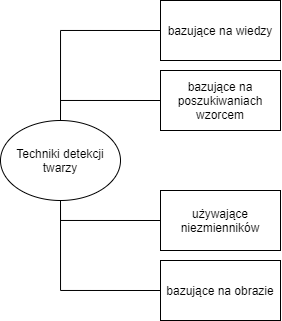
\includegraphics[width=7cm]{techniki-detekcji.png}
	\caption{Techniki detekcji twarzy według Younga.} 
	\label{fig:detectionMethods}
\end{figure}

Charakteryzację każdej z grup \cite{Yang} można przedstawić w następujący sposób:
\begin{itemize}
    \item metody bazujące na wiedzy - wykorzustujące ludzką wiedzę na temat elementów jakie zawiera przeciętna twarz
    \item techniki używające niezmienników - algorytmy skupiają się na zlokalizowaniu cech strukturalnych twarzy, które są niezmienne ze względu na kąt, oświetlenie, pozycję twarzy
    \item metody bazujące na przeszukiwaniu wzorcem - dzięki wielu zgromadzonym wzorcom odnośnie wyglądu twarzy lub jej konkretnych elementów poszukuje się korelacji między owym schematem a obrazem wejściowym
    \item metody bazujące na obrazie - model trenowany jest zestawem obrazów, które zawierają różnorodne ludzkie twarze, przedstawiane w zmiennych warunkach
\end{itemize}
Zagadnienie poruszane w tym rozdziale jest bardzo rozległe, a rozwiązania i algorytmy istniejące na rynku bardzo różnorodne. Większość powstałych implementacji łączy najlepsze cechy z kilku metod, przez co nie ma możliwości przypisania ich do konkretnej klasyfikacji. Ze względu na szeroki zakres tej technologii w dalszej części zostaną opisane dwa wybrane algorytmy, których implementacje zawarte są w bibliotekach umożliwiających wykorzystanie gotowego programu.

\subsection{Schemat działania}
% Algorytmy wykrywania twarzy często postępują w podobny sposób. Większość z nich rozpoczyna swoje działanie od zlokalizowania oczu na obrazie ze względu na ich charakterystyczność. Zdaje się to być najprostszym elementem do wykrycia. \cite{fDetection}

Struktura algorytmu wykrywania twarzy odbywa się dwuetapowo. Początkowym etapem jest wyszkolenie klasyfikatora, którego zadaniem będzie wykrycie twarzy. Następnie potrzebne jest działanie detektora skanującego cały obraz w celu lokalizacji istotnych cech jak oczy, usta, nos czy brwi zawartych w wytrenowanym wcześniej modelu.

Większość algorytmów uzależnia swoją efektywność od wielkości danych, na których został przeszkolony klasyfikator. Trenowanie na dużych zbiorach danych poprawia zdolność algorytmu w trakcie określenia czy na danym obrazie znajduje się twarz. \cite{fDetection}

\subsection{Haar Cascades}
Paul Viola i Michael Jones w 2001 roku zaproponowali technikę wykrywania obiektów opartą o działanie klasyfikatora kaskad Haara (Haar Feature-based Cascade Classifier). Pomimo wysokiej konkurencji ze strony sieci neuronowych, algorytm cieszy się ogromną popularnością po dzień dzisiejszy. \cite{haarCascade}Jego zastosowanie okazało się być przełomem w dziedzinie wykrywania twarzy. 
% Wykrywanie obiektów za pomocą algorytmu opartego o klasyfikator kaskadowy (ang. Haar Feature-based Cascade Classifier) zostało pierwszy raz zaproponowane w 2001 roku przez Paula Violę i Michaela Jonesa.

Działanie tej techniki \cite{haar} łączy ze sobą poniższe koncepcje:
\begin{itemize}
    \item poszukiwanie i wybór najdokładniejszych cech Haara
    \item utworzenie zintegrowanych obrazów w celu szybkiego znalezienia danej cechy
    \item użycie metody sprawnego uczenia Adaboost
    \item zastosowanie klasyfikatora kaskadowego% (nakładanie się, zawieranie w sobie, części wspólne)
\end{itemize}

Jest to podejście oparte o wytrenowanie klasyfikatora kaskadowego na wielu pozytywnych i negatywnych obrazach przedstawionych w skali szarości. Przez pierwszy rodzaj rozumie się zdjęcia zawierające twarze, natomiast jako próbki negatywne określa się zdjęcia, na których nie znajduje się twarz ludzka. Według zaleceń autorów algorytmu obrazy powinny mieć wymiary $24x24$ pikseli.

Pierwszym krokiem działania tego algorytmu jest wydobycie ze wszystkich próbek odpowiednich cech Haara. Cechy te dotyczą zmian wartości kontrastu pomiędzy prostokątnymi grupami pikseli. W tym celu wykorzystuje się tak zwane funkcje Haara.

Są to kombinacje prostokątów  o takich samych wymiarach (ciemnych i jasnych), pozwalające na detekcję konkretnych elementów. Funkcje dzielimy na trzy grupy, ze względu na ilość prostokątów (2, 3, 4) tworzących daną cechę. Na Rys. \ref{fig:haarFeatures} przedstawiono funkcje używane w tym algorytmie, wykorzystywane do wykrywania krawędzii na obrazie (1, 2) oraz prostych (3) i skośnych linii (4).

\begin{figure}[h]
	\centering
	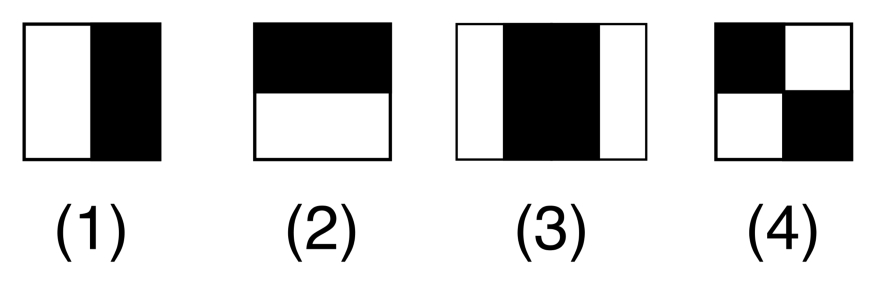
\includegraphics[width=6cm]{haar_features.png}
	\caption{Przykładowe funkcje Haara. \cite{haarCascade}} 
	\label{fig:haarFeatures}
\end{figure}

Każda funkcja Haara przemierza piksel po pikselu danego obrazu. Dla każdego regionu (ciemnego jak i jasnego), który obejmuje owa cecha, sumowana jest wartość pikseli znajdujących się w tych obszarach. Następnie obliczana zostaje różnica między tymi sumami. Na podstawie owej różnicy, która powinna być jak największa, wyszukuje się lokalizację na obrazie, dla której dana cecha jest najbardziej odpowiednia. 


 
Przykładowo, na Rys. \ref{fig:haarNose} użyto funkcji złożonej z trzech prostokątów, o rozmiarze mającym na celu wykrycie oczu. Możliwe jest to poprzez fakt, iż obszar oczu jest ciemniejszy niż obszar nosa znajdujacy się pomiędzy nimi. Cechy Haara są pewnego rodzaju wzorcem, dla którego należy znaleźć najlepsze dopasowanie na obrazie.
 
\begin{figure}[h]
	\centering
	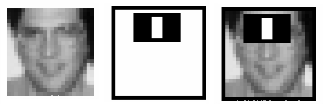
\includegraphics[width=5cm]{haar_nose_feature.png}
	\caption{Zastosowanie funkcji Haara do wykrycia oczu i obszaru nosa.} 
	\label{fig:haarNose}
\end{figure}
 
Próba dopasowania cech Haar'a przechodząc każdy piksel zawarty na obrazie jednocześnie dobierając różne rozmiary danej cechy, wymaga ogromnej liczby działań. Rozwiązaniem jest stworzenie zintegrowanego obrazu. Tym pojęciem nazywamy reprezentację obrazu, w którym dana wartość $(x, y)$ równa jest sumie pikseli znajdujących się powyżej i na lewo od analizowanej lokalizacji (Rys. \ref{fig:integralImage}). Owa reprezentacja pozwala na przyspieszenie obliczeń. Jest to skuteczny sposób obliczenia sumy wartości pikseli dla prostokątnego podzbioru rozważanego obrazu.
 
 \begin{figure}[h]
	\centering
	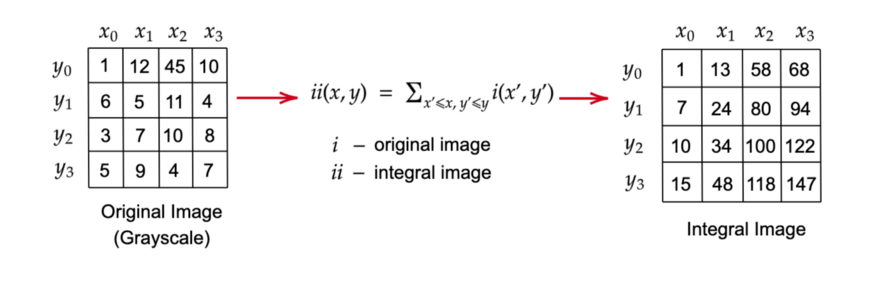
\includegraphics[width=10cm]{integral.png}
	\caption{Konwersja na obraz zintegrowany. \cite{haarCascade}} 
	\label{fig:integralImage}
\end{figure}
 
 
 Kolejnym krokiem jest wybór cech, które są istotne dla konkretnych obszarów. Ten efekt można osiągnąć z pomocą algorytmu Adaboost (Adaptive Boosting), będącego algorytmem uczenia maszynowego służącego do wyboru najlepszych funkcji. Owa technika wzmacniająca, poprzez zastosowanie wszystkich możliwych cech na każdym obrazie treningowym osobno, wybiera te o najniższym błędzie dla danej iteracji. Owy algorytm trenuje silny klasyfikator na podstawie liniowej kombinacji słabych klasyfikatorów.% Słabymi klasyfikatorami nazywa się najlepsze cechy o najniższym poziomie błędu dla danej iteracji. 
 
 Po wyborze najlepszych cech spośród wszystkich możliwości pozostaje etap zastosowania klasyfikatora kaskadowego. Z definicji, działa on wielostopniowo. Cechy wybrane jako kluczowe zostają podzielone na grupy, gdzie każda z nich odpowiada jednemu etapowi działania klasyfikatora. Pierwsze etapy zawierają niewiele funkcji, ale wybrane zostają te najbardziej pewne i charakterystyczne. 
 
Funkcje są nakładane na każde okno o zadanych wymiarach wyodrębniane na obrazie. W przypadku negatywnego rezultatu, tzn niedopasowania jednej z cech sprawdzanych w konkretnym etapie, analizowane okno jest od razu odrzucane. Nie rozważa się dla niego funkcji zawartych w dalszych etapach. Jeśli natomiast okno przejdzie pomyślnie wszystkie etapy działania klasyfikatora kaskadowego zostaje zaklasyfikowane jako obszar twarzy (Rys. \ref{fig:cascadeClasificator}).  
 
   \begin{figure}[h]
	\centering
	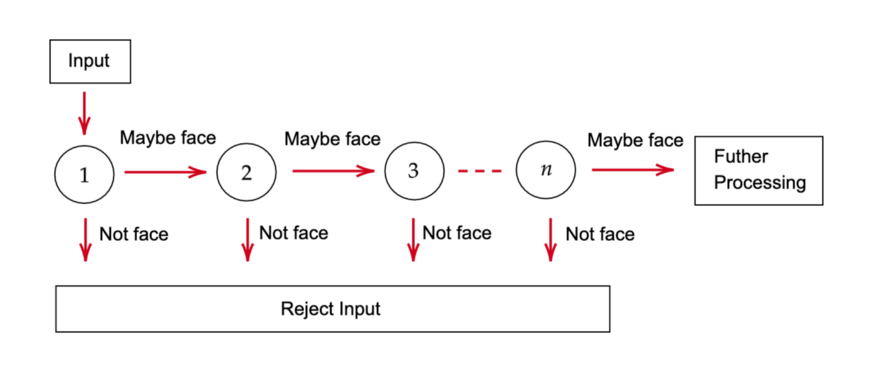
\includegraphics[width=10cm]{haar_train.png}
	\caption{Klasyfikator kaskadowy. \cite{haarCascade}} 
	\label{fig:cascadeClasificator}
\end{figure}

W badniu przeprowadzonym przez autorów algorytmu wybrano 6000 funkcji, które podzielono na 38 etapów klasyfikacji. Liczba cech w każdym z nich nie jest proporcjonalna, wynosi ona kolejno 1, 10, 25, 25, 50 funkcji dla pięciu pierwszych etapów. W początkowych etapach eliminujemy okna, w których nie ma elementówch charakterystycznych twarzy. Oszczędza to zbędnych obliczeń i analiz.

Opisany w tym rozdziale algorytm jest wykorzystywany nie tylko do wykrywania twarzy na obrazach, ale także innego rodzaju obiektów, takich jak zwierzęta, tablice rejestracyjne czy całe ludzkie sylwetki. Jego popularność zdaje się dalej trwać, pomimo odkrycia wielu innych algorytmów działających na podobnej zasadzie. %Cechuje go.. 

% W internecie jest wiele źródeł udostępniających darmowe biblioteki, które zawierają gotowe modele wyrenowanych klasyfikatorów kaskadowych. 


 
 
 
 
 

 
 
 



 
 

\subsection{HOG + SVM}
ten implementuje HOG i SVM


\section{Wykrywanie punktów charakterystycznych}
w sumie no to jesli chodzi o pythona, tooo np te modele od razu tez wykrywaja landmarki jak juz twarz xd too moze ze wzgledu na ich ilosc? jakos porownac czy co, bo iksde w sumie eh joj

\section{Triangulacja Delaunaya}
Poprzez pojęcie triangulacji, w kontekście matematycznym, można rozumieć podział figury geometrycznej na trójkąty, bądź też czworościany (określane jako sympleksy) w taki sposób, aby część wspólna dwóch sąsiadujących trójkątów (czworościanów) była ich wspólną ścianą, wierzchołkiem, bokiem, trójkątem lub zbiorem pustym. \cite{triangulation}

Istnieje wiele różnych rodzajów triangulacji. W przypadku rozważanego w tej pracy algorytmu wykorzystano triangulacje zbioru punktów, do której należy między innymi triangulacja Delaunaya (lub Delone), której nazwa pochodzi od nazwiska autora tejże koncepcji Borysa Delaunaya. 

Triangulacja Delone \cite{tDelone} rozumiana jest jako triangulacja $T$ przestrzeni $R^{n+1}$, którą definiuję się w poniższy sposób.

Jako $T$ określa się podział przestrzeni $R^{n+1}$ na $(n+1)$ sympleksów, z punktami jako wierzchołki, spełniających okreśone warunki:

\begin{enumerate}
    \item każde dwa sympleksy należące do zbioru $T$ posiadają wspólną ściane albo nie są ze sobą połączone w żaden sposób
    \item każdy z ograniczonych zbiorów w przestrzeni $R^{n+1}$ ma część wspólną z ograniczoną liczbą trójkątów ze zbioru $T$
    \item opisując kulę na dowolonym trójkącie ze zbioru $T$ nie natkniemy się na sytuację, gdy wnętrze kuli będzie zawierało wierzchołki z pozostałych sympleksów zawartych w zbiorze $T$
\end{enumerate}

\begin{figure}[h]
	\centering
	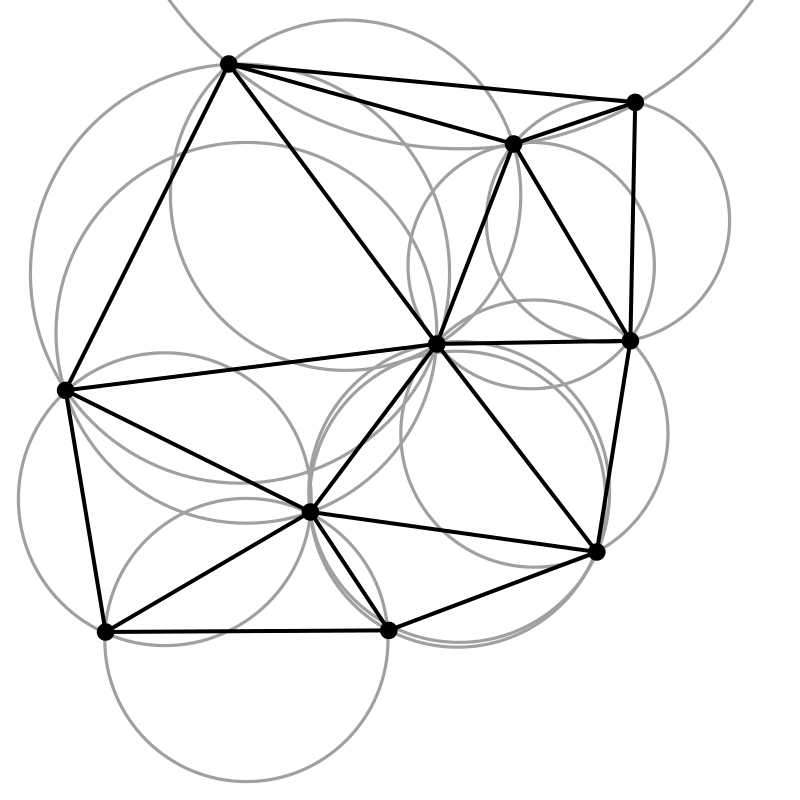
\includegraphics[width=7cm]{triangulation.png}
	\caption{Przykładowa triangulacja Delone dla zbioru punktów. \cite{tDelone}}
	\label{fig:delone}
\end{figure}

Wspominając o triangulacji Delone warto wspomnieć o diagramach Voronoi, które są ściśle powiązane z owym pojęciem. Diagram Voloroi dla zestawu punktów dzieli przestrzeń w taki sposób, że linie podziału znajdują się w równej odległości od punktów sąsiadujących.

Ważną własnością trangulacji Delone jest fakt, iż wraz z diagramem Voronoi tworzy ona graf dualny. Te definicje są powiązane, więc znając trangulację Delone dla zbioru punktów możemy w łatwy sposób obliczyć diagram Voronoi. Dwa trójkąty mające wspólną krawędź w triangulacji umożliwiają odnalezienie krawędzie w diagramie Voronoi. 

Centra okręgów wyznaczonych przez owe trójkąty po połączeniu tworzą daną krawędź. Rys. \ref{fig:voronoi}  przedstawia krawędzie triangulacji (czarne linie) oraz utworzone na podstawie triangulacji komórki Voronoi (czerwone linie).

\begin{figure}[h]
	\centering
	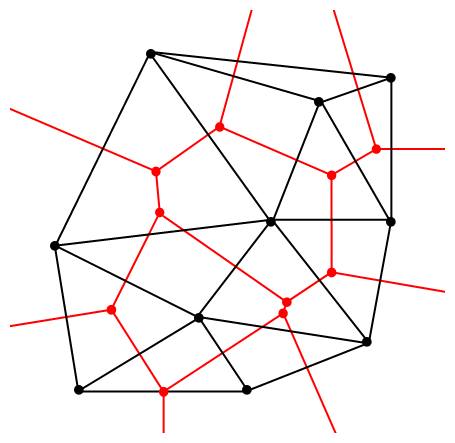
\includegraphics[width=7cm]{voronoi.png}
	\caption{Graf przedstawiający komórki Vornoi oraz krawędzie triangulacji. \cite{tDelone}} 
	\label{fig:voronoi}
\end{figure}

Istotną własnością tej techniki jest fakt, że trójkąty powstałe w wyniku triangulacji nie mają kątów o dużych miarach, co zapewnia przejrzystość wygenerowanych figur. W przypadku zastosowania triangulacji na zbiorze punktów można uniknąć chaosu i nierównomierności.

Triangulacja ma swoje zastosowania w wielu dziedzinach. Wykorzystuje się ją w informatyce, grafice komputerowej czy też geodezji. Technika umożliwia tworzenie skomplikowanych figur, wypełnianie obszarów, wyznaczanie linii przecięcia.

Istnieje wiele różnych algorytmów przeznaczonych do znajdowania trangulacji Delone dla zbioru punktów. Przedstawienie ich w niniejszej pracy dyplomowej nie jest jednak kluczowe. Większość języków programowania dostarcza odpowiednie biblioteki, które posiadają funkcje implementujące takowe algorytmy. 


% Istnieje wiele różnych algorytmów przeznaczonych do znajdowania trangulacji Delone dla zbioru punktów. Nie jest to jednak kluczowe w przypadku niniejszej pracy dymplomowej. W implementacji zostanie użyta odpowiednia biblioteka, która implementuje algorytm triangulacji Delone. 

% W przypadku tworzenia algorytmu animacji awatara istotne jest, aby trójkąty tworzone ze zbioru punktów charakterystycznych były zbudowane w odpowiedni sposób. Trójkąty powstałe w wyniku triangulacji nie będą mieć dużych kątów, co zapewni przejrzystość powstałych figur. W przypadku podziału twarzy na takowe figury unikniemy chaosu, nierównomierności. Właśnie dlatego zdecydowałam się na wybór tejże techniki.


